
%    INSTITUTE OF PHYSICS PUBLISHING                                   %
%                                                                      %
%   `Preparing an article for publication in an Institute of Physics   %
%    Publishing journal using LaTeX'                                   %
%                                                                      %
%    LaTeX source code `ioplau2e.tex' used to generate `author         %
%    guidelines', the documentation explaining and demonstrating use   %
%    of the Institute of Physics Publishing LaTeX preprint files       %
%    `iopart.cls, iopart12.clo and iopart10.clo'.                      %
%                                                                      %
%    `ioplau2e.tex' itself uses LaTeX with `iopart.cls'                %
%                                                                      %
%%%%%%%%%%%%%%%%%%%%%%%%%%%%%%%%%%
%
%
% First we have a character check
%
% ! exclamation mark    " double quote  
% # hash                ` opening quote (grave)
% & ampersand           ' closing quote (acute)
% $ dollar              % percent       
% ( open parenthesis    ) close paren.  
% - hyphen              = equals sign
% | vertical bar        ~ tilde         
% @ at sign             _ underscore
% { open curly brace    } close curly   
% [ open square         ] close square bracket
% + plus sign           ; semi-colon    
% * asterisk            : colon
% < open angle bracket  > close angle   
% , comma               . full stop
% ? question mark       / forward slash 
% \ backslash           ^ circumflex
%
% ABCDEFGHIJKLMNOPQRSTUVWXYZ 
% abcdefghijklmnopqrstuvwxyz 
% 1234567890
%
%%%%%%%%%%%%%%%%%%%%%%%%%%%%%%%%%%%%%%%%%%%%%%%%%%%%%%%%%%%%%%%%%%%
%
\pdfminorversion=4

\documentclass[12pt]{iopart}
\usepackage{graphicx}
\usepackage{amssymb}
\usepackage{enumitem}
\usepackage{xcolor}
\newcommand{\gguide}{{\it Preparing graphics for IOP Publishing journals}}
%Uncomment next line if AMS fonts required
%\usepackage{iopams}  
\begin{document}

\title[]{Closed-loop EEG study on visual recognition during driving}

\author{Ruslan Aydarkhanov$^1$,
Marija U\v{s}\'{c}umli\'{c}$^2$,
Ricardo Chavarriaga$^{3,4}$,
Lucian Gheorghe$^5$,
Jos\'e del R Mill\'an$^{3,6,7}$}


\address{$^1$Medical Image Processing Laboratory,
Center for Neuroprosthetics,
Interschool Institute of Bioengineering,
\'Ecole Polytechnique F\'ed\'erale de Lausanne (EPFL),
Campus Biotech H4,
1202 Geneva,
Switzerland}
\address{$^2$Nissan International SA,
La Pi\`ece 12,
1180 Rolle,
Switzerland
}
%\address{$^3$Zurich University of Applied Sciences, ZHAW,
%InIT Institut of Applied Information Technology,
%Ob. Kirchgasse 2,
%8400 Winterthur,
%Switzerland}

\address{$^3$\'Ecole Polytechnique F\'ed\'erale de Lausanne (EPFL),
Campus Biotech H4,
1202 Geneva,
 Switzerland}

\address{$^4$ZHAW Datalab, Zurich University of Applied Sciences, Winterthur, Switzerland
 }

\address{$^5$
Advanced Materials and Processing Laboratory, Nissan Research Center, Nissan Motors Co. LTD, 1,
Natsushima, Yokosuka-shi, Kanagawa-ken, 237-8523, Japan
}
\address{$^6$Dept. of Electrical and Computer Engineering,
The University of Texas at Austin,
Austin, TX 78712,
USA}
\address{$^7$Dept. of Neurology,
The University of Texas at Austin,
Austin, TX 78712,
USA}
\ead{ruslan.aydarkhanov@epfl.ch}
\vspace{10pt}
%\begin{indented}
%\item[] August 2017
%\end{indented}

\begin{abstract}
\textit{Objective.} 
In contrast to the classical visual BCI paradigms
which adhere to a rigid trial structure and restricted user
behaviour, EEG-based visual recognition decoding during
our daily activities remains challenging.
The objective of this study is to explore 
the feasibility to decode the EEG signature 
of visual recognition in experimental conditions
promoting our natural ocular behavior 
when interacting with our dynamic environment. 
\textit{Approach.} 
In our experiment, subjects visually search for
a target object among suddenly appearing objects 
in the environment while driving a car-simulator.
Given that subjects exhibit an unconstrained overt 
visual behaviour, we based our study on 
eye fixation related potentials (EFRP).
We report on visual behavior and single-trial 
EFRP decoding performance (fixations on task 
related vs. distracting objects).
In addition, we demonstrate the application
of our approach in a closed-loop BCI setup.
\textit{Main results.}
By integrating decoding probabilities of multiple EFRP
the online accuracy reached 0.37 on average in
identifying one target out of four board types.
Using the acquired data, we performed a comparative study
of classification algorithms and feature spaces in
a simulated online scenario. The EEG approaches yielded
similar moderate performances not higher than 0.6 AUC,
yet significantly above the chance level.
In addition, the gaze duration (dwell time) appears
to be an additional informative feature in this context.
\textit{Significance.}
These results show that visual recognition of sudden events
can be decoded during active driving. 
It lays a foundation for assistive and recommender systems
based on driver's brain signals.
\end{abstract}

%
% Uncomment for keywords
\vspace{2pc}
\noindent{\it Keywords\/}: Brain-computer interfaces, Electroencephalography, Eye tracking, Driving,
Visual recognition
%
% Uncomment for Submitted to journal title message
%\submitto{\JPA}
%
% Uncomment if a separate title page is required
%\maketitle
% 
% For two-column output uncomment the next line and choose [10pt] rather than [12pt] in the \documentclass declaration
%\ioptwocol
%



%There exist various well-established EEG-based BCI paradigms which
%provide a high performance and rely on such phenomena as
%Sensorimotor Rhythms (SMR), Steady-State Evoked Potentials (SSEP),
%or Event-Related Potentials (ERP) and others \cite{hwang_eeg-based_2013}.
%For each paradigm a specific data processing and feature
%extraction steps are required \cite{lotte_review_2018}.

\section{Introduction}
\label{sec:intro}

%Decoding of neural and behavioral correlates 
%of visual recognition is complex in everyday life.
%%Driving is a good example of daily activity in real life
%%where BCI can enhance the driver's experience.
%One of the common everyday activities is driving
%which is a complex activity involving 
%a range of neural processes from motor control
%to visual information processing, thus illustrating
%many BCI challenges in real world application.

Brain-computer interfaces (BCI), especially those based on 
non-invasive electroencephalogram (EEG) signals, are not only
proving their value as assistive tools for people 
with disabilities
\cite{birbaumer_spelling_1999,wolpaw_control_2004,holz_braincomputer_2013,leeb_towards_2015,saeedi_long-term_2017,perdikis_cybathlon_2018}
and potential rehabilitation tools for
neurological patients
\cite{ramos-murguialday_brain-machine-interface_2013,pichiorri_braincomputer_2015,biasiucci_brain-actuated_2018,cervera_braincomputer_2018},
but also open opportunities 
to augment interaction for users without disabilities \cite{zhang_eeg-based_2015,khaliliardali_action_2015,chavarriaga_decoding_2018}. In this
later respect, a promising possibility is to decode neural
correlates of perceptual and cognitive processes while people
overtly interact with real-world environments
\cite{uscumlic_iterative_2013,jangraw_neurally_2014,haufe_electrophysiology-based_2014}.
In this work, we explore the feasibility to decode visual recognition
from EEG in experimental conditions mimicking our
daily activities which involve overt visual search. In particular,
we performed a study on visual BCI in
driving -- aiming at decoding visual recognition
while a driver is primarily engaged in controlling a car simulator,
actively exploring the visual environment to complete a visual search task.

Previous works have reported certain EEG signatures of visual recognition in simple, well-controlled experimental setups
\cite{gerson_cortically_2006,krusienski_toward_2008,rosenthal_evoked_2014,jangraw_neurally_2014}.
The classical restrictive conditions require that
the stimuli are static and undergo sharp
transitions (e.g. flashing) as well as 
subjects sit still in front of a screen \cite{krusienski_toward_2008}. 
In such experiments with an oddball paradigm 
where subjects had to recognize
rare targets stimuli in a sequence, the recognition process
is reflected in EEG as the well-known P300 component of Event-Related Potential (ERP).
P300 is a positive deflection in parietal region which occurs
approximately between 250 and 500 ms after the stimulus onset \cite{polich_updating_2007}.
This signal has been successfully used in various BCI applications such as
P300-based speller because of high decoding performance.
With the typing speed of 10 characters per minute \cite{rezeika_braincomputer_2018},
the home use of such spellers may improve the quality of life
of people with severe motor disabilities, such as ALS
\cite{sellers_brain-computer_2010,holz_long-term_2015,wolpaw_independent_2018}.
For people without motor impairments, however, this setup and typing performance does not bring much value.

Car drivers are exposed to a richer environment and need to constantly interact with it
by controlling the car, visually exploring the surrounding and
planning upcoming actions. 
Successful decoding of visual recognition in free viewing tasks
would open space for BCI application for healthy users
by providing them assistance and recommendations.
A hypothetical application scenario may include
the driver's recognition of road signs of a particular target category, e.g. parking.
The driver's interest in parking signs decoded from the EEG
will allow to provide timely recommendations for the nearest parking.

In free viewing conditions, people need to fixate
or track moving objects to perceive them in all details.
Fixations evoke a type of ERP called Eye Fixation Related Potentials (EFRP)
as opposed to external events in more classical ERP designs.
Early EEG deflections in EFRP reflect the processing of low-level features 
of visual input projected from the retina to the occipital lobe of the cortex
and are manifested mainly in high-amplitude 
of the P100 component, also referred to as lambda component \cite{evans_further_1952}.
Later EEG deflections in EFRP resemble the P300 component in the oddball paradigm \cite{brouwer_distinguishing_2013}.

Visual stimuli used in previous ERP and EFRP studies range from simple geometric shapes
in static scenes, to static natural images or dynamic
scenes with geometric shapes \cite{uscumlic_active_2016, devillez_p300_2015}.
Only a few attempts on decoding ERP or EFRP in videos or virtual reality (VR) simulations
have been reported, e.g. \cite{rosenthal_evoked_2014,jangraw_neurally_2014}. 
%\textcolor{red}{Limitations of these studies
%and motivate my study.
%Explain that the used experimental conditions do not correspond to real world environment.
%There is no real driving involved as a primary task STUDY 1.
%The authors sped up the action video to clearly define the relevant
%event time STUDY 2.}
However, the experimental conditions in those studies did not fully
reflect the real-world dynamics.
For instance, in human action recognition from a cartoon animation, the video playback was sped up
to limit the time of the recognition process, and other experimental
settings made unnecessary to utilize eye-tracking 
as it would have been the case on more natural setups \cite{rosenthal_evoked_2014}.
%Examples of actions
%include a person looking at his watch or entering the scene.
%No eye-tracking was used and ERP was analyzed due to occurrence of 
%a single salient event on the video \cite{rosenthal_evoked_2014}.
The classification performance of Target vs Non-Target event reached average AUC $> 0.8$.
In another study involving maze navigation, subjects experienced fast autonomous driving
and had to press a button whenever the car in front braked suddenly \cite{jangraw_neurally_2014}.
The braking task required constant monitoring of the car in front, leading
to a brief visual attendance of the stimuli. It resembled the attentional load
of real driving, however, an unnaturally high speed and lack of full car control
limit the transfer of the results to real driving.
The classification performance based on single EFRP 
was around $0.65$ AUC on average across subjects.

%In our study subjects perform visual recognition task while primarily engaged
%in active driving in a car simulator.
%The subject are faced with natural radially expanding optic flow.
%We study EFRP
%while driving and
%facing optic flow
%yet we ensured that recognition happens upon the fixation by introducing pop up effect.

In this paper we report a study on visual recognition decoding during driving
in a car simulator based on the Eye Fixation Related
Potentials and visual behavior. 
In our study 13 subjects visually attended billboards along the roads
while primarily engaged in active driving through
an urban environment with a natural speed of $\thicksim$ 80 km/h. 
We introduced, nevertheless, certain limitation concerning 
the stimuli presentation.
The boards were invisible until the driver gets close enough,
then they pop out at a random locations above the sidewalks.
Such popping up of the board ensured 
that once drivers gaze at a board, they can recognize the content.
Otherwise, there would be 2 challenges in decoding
visual recognition due to fixations on distant
and poorly recognizable boards:
1) to locate the recognition timing within long attendance,
2) to select one of multiple returning fixations when the recognition occurs.
The latter challenges collecting clean data while the former challenges
the EFRP decoding itself.

The experiment consisted of 2 phases: offline and online.
The goal of the offline phase was two-fold: (1) to analyze behavioral
and neural correlates of visual recognition and (2) to gather data to train
a classifier to be used in the online phase.
Then we conducted the online phase to study the performance
of the decoder in a closed-loop setting and, as a major objective, to verify
the feasibility of the corresponding BCI application.

Our protocol closely resembles the real-life scenario of traffic sign
recognition on the roads. In the application, 
the BCI system that decodes the cognitive response on the target sign
recognition can be integrated into the advanced driver-assistance system
(ADAS) of the car.
In this case the target is naturally chosen by the driver
according to the current driving situation. 
The accurate decoding of the selection of target traffic signs 
from the driver’s brainwaves can shed light on the driver’s intentions
and goals, from which the ADAS system could derived useful 
recommendations and assistance.

%The accurate
%decoding of the target traffic signs from the driver's mind
%can shed light on what the driver's intentions and needs
%and can be utilized for useful suggestions and recommendations.

%Although subjects followed
%the objects moving on the screen,
%we could analyze their eye behavior by approximating smooth pursuit
%with consecutive fixations combination.


%Brain Computer Interfaces (BCI) proved their potential utility 
%by successfully passing tests in controlled laboratory conditions.
%One of the remarkable examples is P300-based spellers
%which allow to type up to 10 characters per minute \cite{rezeika_braincomputer_2018}.
%The home use of such spellers can improve the quality of life
%of patients with strong motor disabilities, such as ALS \cite{sellers_brain-computer_2010,holz_long-term_2015}.
%However, bringing BCI to everyday life for healthy people
%remains a challenge.

%A classical P300-based speller presents a static matrix of symbols on a screen.
%The symbols are highlighted in groups (i.e. column-wise and row-wise)
%by flashing regularly. The users pay attention on the screen and 
%do a mental evaluation of whether the target symbol is highlighted or not.
%At each flash an Event-Related Potential (ERP)
%is elicited, and when the user believes that the target is active
%the ERP will contain P300 component.
%To reduce the noise in the signals the users are instructed to limit their body as well as
%eye movements by staring in the middle of the screen.

%The real world is more diverse and more dynamic than traditional
%P300-based experimental protocols. So the time to evaluate
%the visual input can vary which is reflected in the ERP waveform \cite{arico_evaluation_2013}.
%Numerous attempts were done to close this gap and investigate
%the limitations to detect P300 under more challenging conditions
%which includes recognition of dynamic or semantically
%rich stimuli as compared to alphabet characters \cite{rosenthal_evoked_2014}.
%Additionally, natural environment does not provide regular flashing stimulation.
%Instead, it is sampled by free visual exploration with free eye movements.
%There are three major types of eye movements: saccades, fixations
%and smooth pursuit. The clear and sharp perception of visual input
%is only possible during fixations and smooth pursuit.
%Fixations trigger a type of ERP called Eye Fixation Related Potentials (EFRP).
%Although P300 was successfully detected within EFRP,
%it 


%P300 is a reflection of a cognitive process of stimulus evaluation and
%categorization. Its application has potential to go beyond the selection from 
%a limited set of stimuli. P300 can be monitored and detected during execution
%of everyday tasks. For example, driving a car provides a suitable context
%for this type of BCI application. Detection of recognition of critical objects
%or traffic events will give a valuable information for the Advanced
%Driving Assistant Systems (ADAS). Various paradigms were developed
%to investigate decoding performance of EFRP-based P300 during simulated driving.
%For passive driving task which require only brake input from the driver
%the P300 decoding can achieve above chance level for half of the participants \cite{jangraw_neurally_2014}.
%In this paper we address the P300 decoding during active simulated driving with automatic gear.




\section{Experimental setup and protocol}
\label{sec:protocol}


\begin{figure}[!t]
    %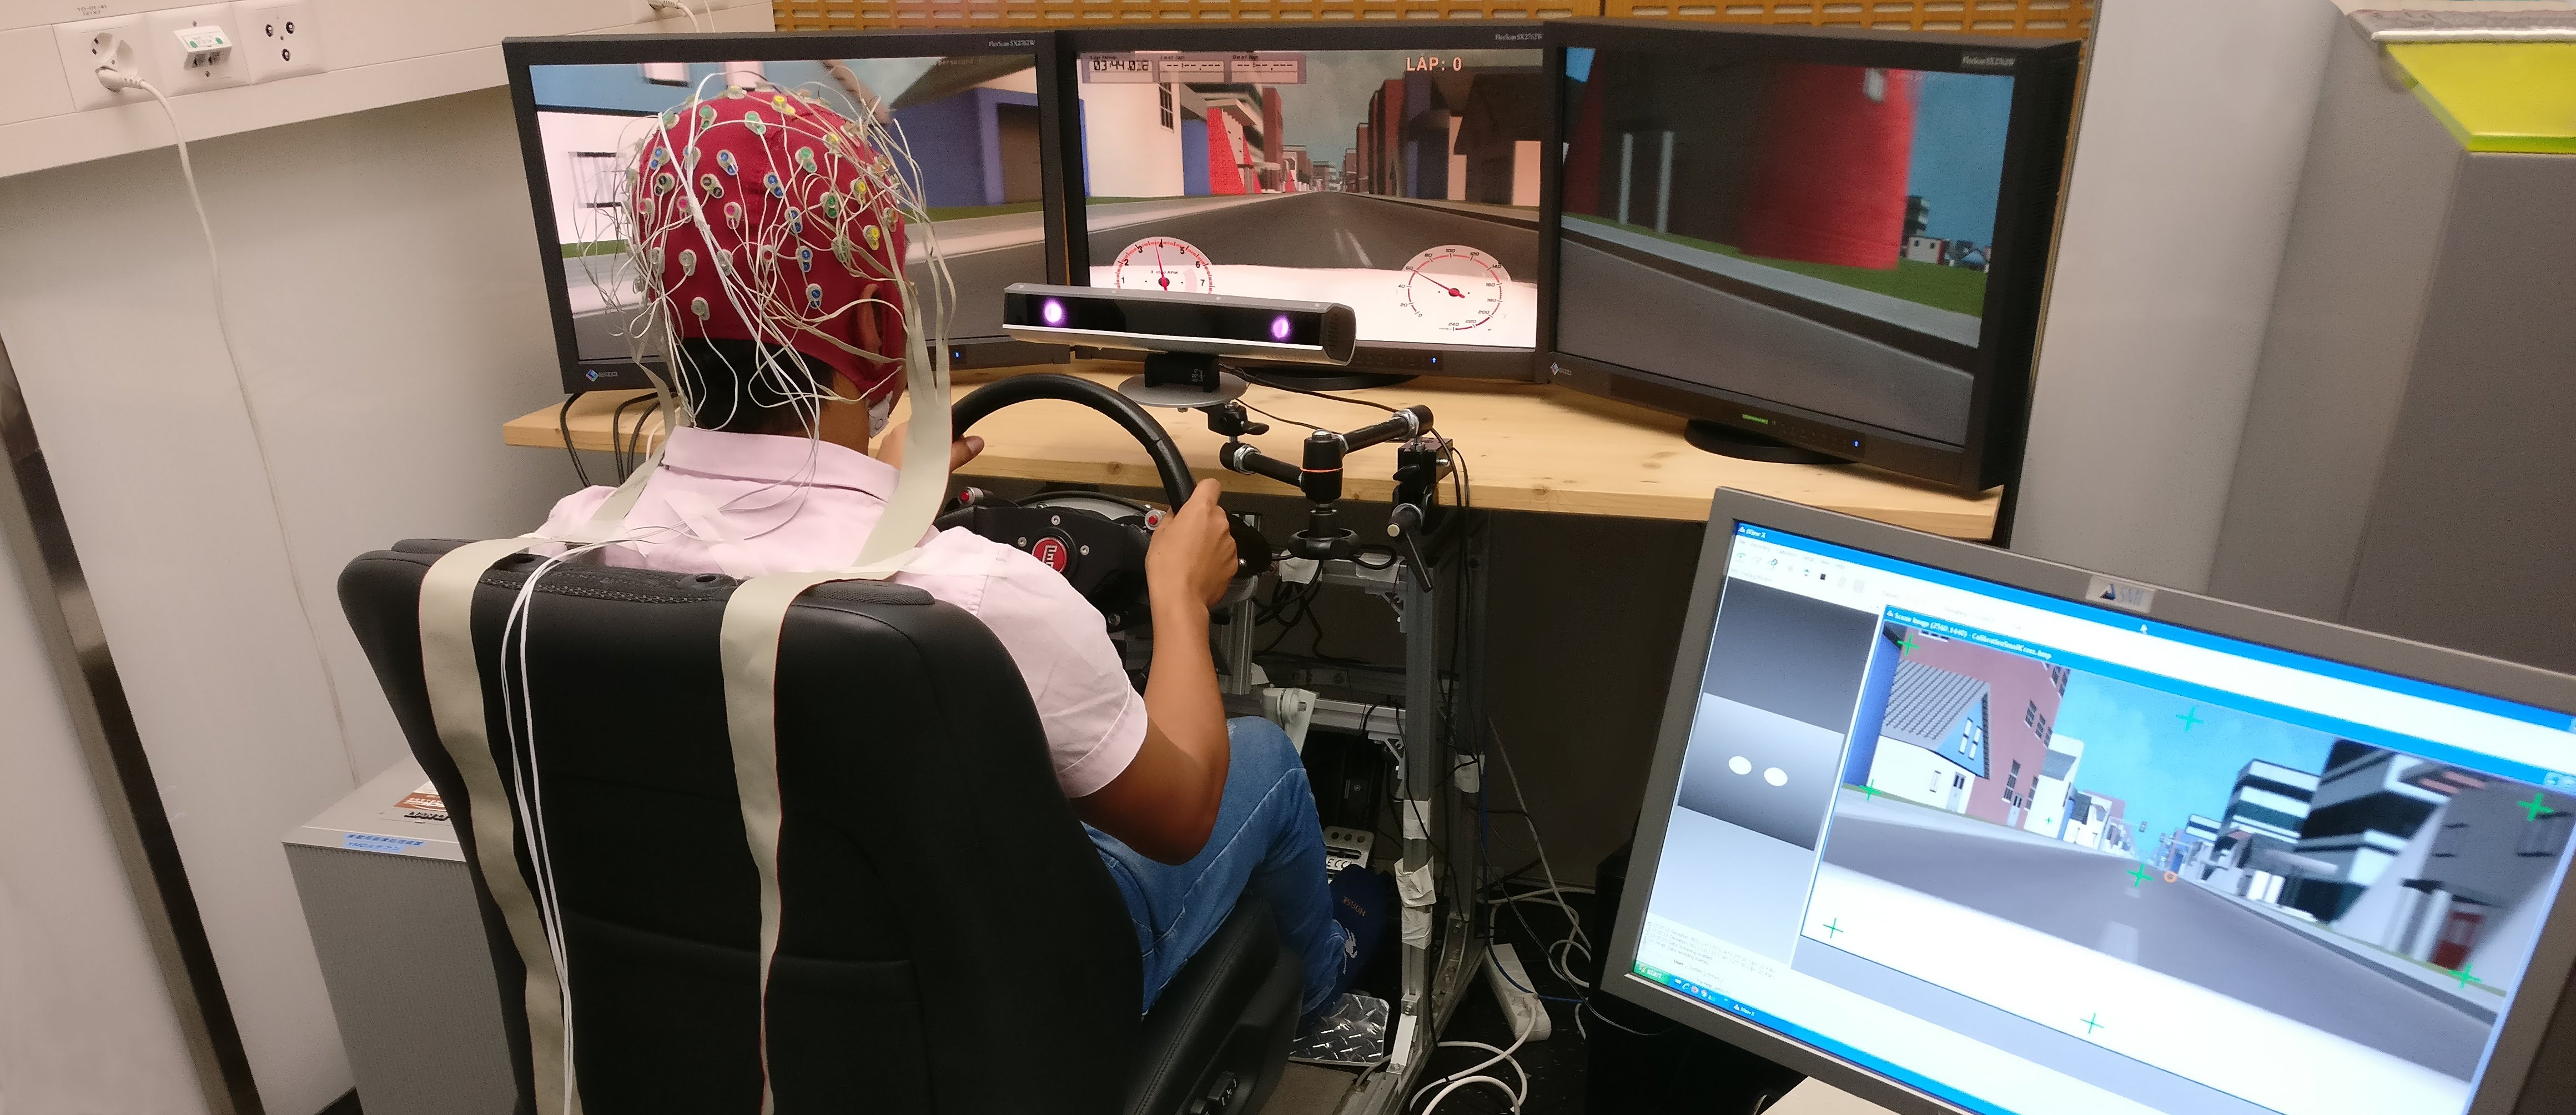
\includegraphics[trim={0cm 0cm 0cm 0cm},clip,width=0.6\columnwidth]{../images/Driving-photo.jpg}
    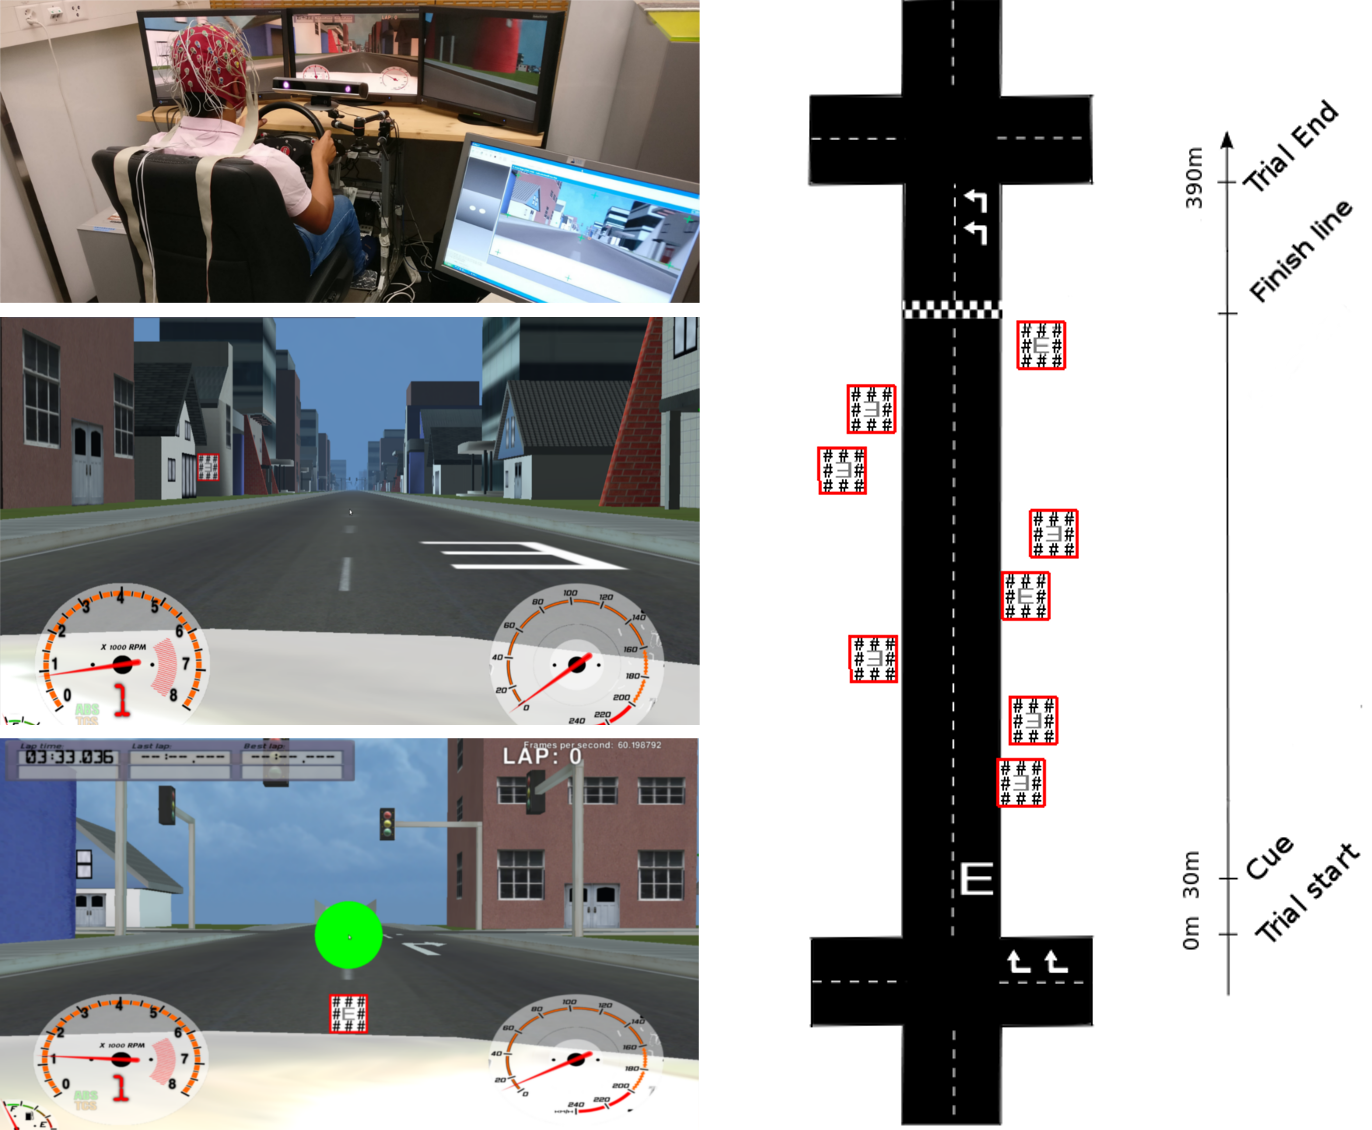
\includegraphics[trim={0cm 0cm 0cm 0cm},clip,width=0.9\columnwidth]{../images/setup_protocol3.png}
    \caption{Visualization of the protocol.
        Top left: The experimental setup with driving simulator (chair and 3 3D screens), 
        Eye-tracker and subject with EEG cap.
        Middle left: screenshot from the beginning of the road with the cue on the floor
        and the first board on the left-hand side.
        Bottom left: screenshot with the online phase feedback for correct decoding, i.e.
        the 2D board at the bottom of the screen and a green circle.
        Right: schematic drawing of one road with the target cue, boards and finish line.
    }
\label{fig:setup}
\end{figure}

\subsection{Data collection}
%We had 13 volunteers (3 female) with the average age of 28.
%Experiment lasted 3 hours including the set up (\~1h), the offline phase (\~45 min),
%the break (\~30 min) and the online phase (\~45 min).

13 volunteers (age of 28 $\pm$ 6, 3 female) participated in the study.
Experiment lasted 3 hours including the set up ($\thicksim$ 1 h), the offline phase ($\thicksim$ 45 min),
one pause period ($\thicksim$ 30 min) and the online phase ($\thicksim$ 45 min).
The extended pause period was necessary to process all the data
from the offline phase and to train the classifier for the online phase.
The offline phase consisted of 3 runs through the city  whereas the online
phase could comprise from 3 to 5 runs depending on the available time
and subject's fatigue.
One run included 20 roads with 12 boards each resulting in 240 boards per run.
Before each run the subjects were asked to move their eyes up-down and left-right
for one minute in order to collect the data for eye movement artifact removal.

The EEG was acquired with BioSemi ActiveTwo system with 64 electrodes at 2 kHz sampling rate.
Additionally, we recorded 3 EOG channels to collect the eye movement data:
two electrodes next to the outer canthi of the eyes and one above the nasion.
%The EEG data was captured and saved on the laptop. The real time processing
%of EEG in online phase was done on the same laptop.
The real time processing
of EEG in online phase was done on a dedicated computer.

The eye gaze was recorded with the SMI RED Eye tracking system 
with sampling rate of 120 Hz.
The chair and eye tracker positions were adjusted for each subject.
The eye tracker
was calibrated with 13 points once after the EEG setup and before beginning of 
the experiment.

The driving simulator logged the car location in the virtual environment,
the controllers state (gas and brake pedals, steering wheel,
buttons on the wheel)
and the 2D position of boards on the screen at a sampling rate
of 256 Hz. In order to synchronize the data acquisition on three separate machines
(EEG, eye tracking and driving simulator) at different sampling rates,
a square pulse of 4 Hz was generated by the driving simulator and sent 
to the eye tracker through TCP connection and to BioSemi through the parallel port.

\subsection{Driving simulator}
%Our system is based on the driving simulator previously used for
%EEG-based BCI experiments \cite{khaliliardali_action_2015,zhang_eeg-based_2015}.
%We extend the protocol published in \cite{renold_eeg_2014}.
In our study we used the driving simulator previously used in
\cite{khaliliardali_action_2015,zhang_eeg-based_2015,renold_eeg_2014}.
It allows for immersive driving experience through the utilization
of real Nissan driving chair with steering wheel and two pedals (gas and brake).
The simulated car has automatic transmission which excludes actions for
manual gear shift.
The visual input is provided with three 3D monitors which create multiple renders for
different angles. The virtual environment is implemented using
the open source driving simulator project VDrift. % \cite{noauthor_about_nodate}.
The environment resembles a regular grid city with static objects, i.e.
building, traffic lights, fields. The task-related objects include
direction indications on the road, target cue, boards with symbols
and finish lines (Figure \ref{fig:setup}).


%\begin{figure}[!t]
    %\includegraphics[trim={0cm 0cm 0cm 0cm},clip,width=0.6\columnwidth]{../images/Target}
    %\caption{Protocol}
%\label{fig:protocol}
%\end{figure}

\subsection{Tasks}
The experimental session had 2 phases: offline and online.
The data collected in the offline phase allows to train a classifier
which is used in the online phase to provide the feedback on the decoding results.
In both phases, the subject is instructed to drive through the city while
following indications left or right turn at the crossings (Figure \ref{fig:setup}).
In the beginning of the road segment a symbol (the cue) is depicted
on the ground. Subjects must memorize and search for it among
the boards appearing through the road segment.
Subjects are asked to count the number of boards with the target symbol in each segment. 
To keep subjects engaged in the task, they have to
report the number of targets in the offline phase or observe a
feedback from the decoder in online phase of the experiment
after they cross a finish line at the end of each road.

We included empty roads where subjects has no additional tasks 
except driving, allowing them to rest from the visual recognition task.
In total, a quarter of the roads were empty.

\subsubsection*{Offline phase.}
After crossing the finish line the subject presses 
a button located at the steering wheel as many times
as the number of target boards he/she counted along the current road.

\subsubsection*{Online phase.}
In the online phase we want to estimate the system's performance
in detecting the target symbol (1 out of 4) among all presented
symbols (see Section \ref{sec:stim}). 
After crossing the finish line the board with predicted target is rendered
at the bottom of the screen as a 2D object (Figure \ref{fig:setup}). 
Subjects are instructed to pay
attention to this feedback.
The online phase resembles a closed-loop interaction because
the subjects perceive the decoder result shortly after
looking at the stimuli, within 15 seconds after the first board on the road.


\subsection{Stimuli presentation}
\label{sec:stim}

\begin{figure}[!t]
    
\includegraphics[trim={0cm 0cm 0cm 0cm},clip,width=0.80\columnwidth]{../images/Stimuli.png}
    \caption{The boards with the used symbols. In offline phase we used only boards 
        with symbol E and flipped E whereas in online phase we used all 4 boards.}
\label{fig:boards}
\end{figure}

\subsubsection{Stimuli visibility.}
The board presentation is carefully adjusted to guide visual behavior of subjects.
First of all, boards are invisible unless the driver approaches them
close enough making them to pop up.
Their positions are generated using the following rules.
The boards appear along the road at an equal distance between them, 
randomly on either side of the road above the sidewalks
with a maximum of 2 boards
on the same side in a row  (e.g., 2 boards on the left in Figure \ref{fig:setup}). The number of boards on left
and right sides are balanced. Since the pop up distance was greater
than the distance between the boards along the road, multiple
boards from the same side were visible in the same time,
so their horizontal and vertical position were adjusted to avoid
the overlap for the driver view.

The maximum speed of the car was limited to 80 km/h to ensure 
that all the targets
can be attended. The subjects were allowed to slow down if it is necessary
to attend all the boards and count the targets.
Nonetheless, all the subjects practiced until they felt comfortable 
with completing the recognition task at the maximum speed
during the EEG setup.
Due to constant speed and regular placement of the boards, the boards
popped up at a regular pace with 900 ms period.

\subsubsection{Stimuli content.} In order to link the perception of the symbols on the board
with the eye fixations, the recognition by
peripheral vision must be avoided. Therefore, the target and distracting
symbols were similar and surrounded by the \# character to create
a crowding effect and force the foveating on the main symbol
as done in previous studies \cite{kamienkowski_fixation-related_2012}.
Additionally, we added a bright red border around the board similar 
to the traffic signs
to create a contrast with the environment and facilitate
their identification (Figure \ref{fig:boards}).

\subsubsection*{Symbols in offline phase.}
In the offline phase one of the two symbols were depicted on each board:
E and $\exists$.
One of them was randomly chosen as a target per road segment
and was presented as the cue
at the beginning of the road. There were 2-4 targets out of 12 boards
on each road with the average fraction of targets of 0.25 in total.

\subsubsection*{Symbols in online phase.}
To allow equal accumulation for each symbol by keeping
a low fraction of targets,
we introduced 2 more symbols resulting into 4 symbols in total.
There were between 2 and 4 boards of each symbol resulting into 12 boards on the road.
Only one of them was a target on each road. Therefore, the fraction
of targets was 0.25 on average as in offline phase.


To decode the target at the end of the road each EFRP associated to the
symbol attendance
is assigned a probability to belong to the target class.
At the end of the road segment the probabilities
of all EFRPs are aggregated symbol-wise by averaging.
The symbol that has the highest probability of a target class
is selected as a predicted target.
Therefore, to allow equal accumulation on average for each symbol 
we increased number of symbols to four.
Each symbol appears between 2 and 4 times
resulting into 12 boards on the road.
The fraction of targets is 0.25 in total.



\begin{table}
    \centering
    \caption{The protocol differences between offline and online phases.}
    \begin{tabular}{l | c | c}
        \hline 
        & Offline & Online \\
        \hline 
        Types of boards & 2 & 4 \\
        \hline
        Task & \shortstack{Count silently \\ Button press at the end} & \shortstack{Count silently \\ Observe the feedback} \\
        \hline 
    \end{tabular}
    \label{tab:OffOn}
\end{table}


\section{Methods}
\label{sec:methods}
%\subsection{Performed analyses}
Our analysis of EEG and behavioral data, as well as visual
recognition decoding, has different objectives in the offline and online phases.
The offline phase is necessary for collecting good quality data
for training a classifier to be used in closed-loop during the online phase
and to estimate its performance. However, it also allows us 
to study EEG correlates of visual recognition and  perform a
comparative study of different classifiers.

The online phase allows the estimation of the closed-loop BCI
application performance.
In the online phase, we apply a single decoding approach. 
In order to make a comparative analysis of different
decoding approaches under online conditions we also performed a simulated online analysis. 

\subsection{Fixation extraction and analysis}
There exist numerous methods to extract eye movement events
from the eye gaze direction.
We used a more robust and accurate method of 
Identification by 2-Means Clustering (I2MC)
\cite{hessels_noise-robust_2017}
for the offline phase data.
In the online phase and simulated online analysis,
we used Identification by Dispersion-Threshold (IDT), a simpler and
easy to implement for real-time processing \cite{salvucci_identifying_2000}


\subsubsection*{Offline phase.}
We relied on the I2MC implementation provided by the authors of the method
using the default parameters.
The main idea behind this method is to find the transition between two consecutive fixations
by applying 2-mean clustering in a sliding window manner.
During a fixation the eyes do not move so if we can clearly detect
2 clusters of gaze direction within the sliding window
it means that they correspond to two fixations.
This method is more precise and robust to noisy outliers which
allows to obtain a training dataset of higher quality.

\subsubsection*{Online phase.}
Since the available implementation of I2MC method cannot be applied 
in real time to extract eye fixations,
we used the Identification by Dispersion-Threshold (IDT) 
supplied with our eye tracking system. Fixation in IDT is extracted
when the signals lies within the dispersion thresholds for at least a minimum fixation duration.
It requires two parameters: we used 100 ms for the minimum fixation duration
and 200 pixels for the maximum dispersion.

\subsubsection*{Simulated online phase.}
The same procedure for fixation extraction is applied as in the online phase.

\subsubsection*{Fixation analysis.}
\label{sec:fixanal}
The P300-like components of cognitive response are stronger when the stimulus is perceived and recognized
for the first time \cite{devillez_p300_2015}. 
We assume that subjects categorized the symbol at the first
attendance so we use only the first fixations on the boards for our analysis.
As mentioned in Section \ref{sec:stim}, the popping up effect is introduced 
and the boards are specially designed to ensure that
recognition takes place near fixation on the symbol.

The visual input during the task is dynamic. Due to driving through
the virtual environment the objects, including the boards, are also moving on the screen.
So we assume that most of the board attendances are done with
smooth pursuit rather than fixations. 
To the best of our knowledge, there is no available algorithm for efficient
extraction of smooth pursuit for eye movement data sampled at 120 Hz.
The only consequence of 
extracting fixation from smooth pursuit is that a single smooth pursuit
may be oversegmented into multiple fixations.
For the sake of our analysis, we do not need to differentiate between
fixations and smooth pursuit movement. The onset of first fixation on a board
will coincide with the onset of smooth pursuit.

Each detected fixation was assigned to a target board, a non-target board or non-board.
Because (1) the visual span for text reading extends up to several degrees, 
(2) the boards were moving and (3) eye tracking data were noisy,
we applied the following approach to assign the boards
to fixations. For each eye gaze sample, we estimate the probability of
fixating eyes on the center of the board according to a normal distribution.
After averaging log-probabilities across the fixation time window we apply a hard
threshold to assign the fixation to a board or a non-board category.
This procedure was implemented in the analysis of the data.
The real-time assignment of fixations on boards in online phase was
modified for computational efficiency. It was based
on the first 100 ms after fixation onset and
used on the average fixation direction within 100 ms.

For the behavioral analysis we estimate 
the dwell time -- the uninterrupted time which the driver spent looking at a board.
The dwells were created
by merging all the fixations on the same board with inter-fixation interval 
between them below 50 ms.
For the sake of a valid comparison between offline and online phases 
in behavioral analysis we used IDT method to extract fixations.



\subsection{EEG processing}
\subsubsection*{EEG processing of offline data.}
All the EEG and EOG were downsampled from 2 kHz to 256 Hz
using FIR antialiasing lowpass filter
and further filtered non-causally with a Butterworth band-pass filter
of order 4 within the band [1, 10] Hz.
Due to low conductivity of the skull and the skin,
EEG signal is spatially smoothed so a high contrast between nearby channels
is a result of noise and movement artifacts. We remove this noise
by keeping only low spatial frequency components after decomposition EEG with SPHARA \cite{graichen_sphara_2015}.
Horizontal and vertical components of eye movement were estimated which allowed
to remove the eye movement artifacts from EEG using multiple regression 
as in \cite{schlogl_fully_2007} using only horizontal and vertical 
components as well as the intercept.
The coefficients of multiple regression were estimated from the 
one-minute session of eye movements before the corresponding run.
Then the signal is spatially
filtered with common-average-reference (CAR). 

\subsubsection*{EEG processing in simulated online analysis.}
The EEG processing was identical to the offline analysis
except for the eye movement artifacts removal.
The multiple regression model was obtained from offline data.

\subsubsection*{EEG processing in online analysis.}
The closed-loop interaction in the online phase required real-time processing.
SMI system provides
a real time eye fixation detection. The fixations were buffered
by a parallel process within the driving simulator, matched with the boards,
and a trigger was sent to the BioSemi system 3 s after the onset of each the fixation
on a board. We choose 3 s delay because we apply non-causal filter on EEG data
and need to diminish the edge effect of the backward filter pass.
EEG processing  was identical to the offline procedure
except for 2 steps:
\begin{itemize}
    \item the spectral filtering was done on a 5 s buffer of data,
        approximately around [-2, 3] s around the fixation onset;
    \item the eye movement artifacts were removed based on the multiple
        regression coefficients trained with offline phase eye movement data.
\end{itemize}

\subsection{Decoding approaches}
To decode visual recognition from EEG signals we extracted the epochs
around the fixation onset -- EEG segment between
200 ms to 1000ms  after the fixation onset.
In addition, we extracted dwell time as eye-gaze based features to detect
visual recognition (see Section \ref{sec:fixanal}).
We investigate and compare different decoding approaches which consist of 
various feature sets and classifiers.

\subsubsection*{Offline and simulated online decoding.}
For the offline analysis we chose the following combination of features and classifiers:
\begin{itemize}
    \item \textbf{PLR-Waveform}. Penalized logistic regression (PLR) trained on waveform features (i.e. the signals
        value at each channel and time point) after reducing
        the dimensionality with PCA. Only the components which explain 90\% of variance
        are kept. 
    \item \textbf{PLR-Dwell}. PLR trained on dwell time on the boards.
    \item \textbf{PLR-Combined}. PLR trained on the combination of waveform features with dwell time. We concatenate
        the two feature sets before applying PCA to keep 95\% of variance. Since the dynamic
        range of dwell time in ms is greater than the one of EEG in uV, most of the dwell time information
        is projected into the first component and kept after the transformation.

    \item \textbf{RF-Waveform}. Random forest trained on waveform features. We use 100 decision trees and
        with maximum depth of 5.
    \item \textbf{PLR-Riemann}. PLR trained on Riemannian features from simple EEG epochs.
        To build Riemannian features we
        estimate spatial covariance matrix with shrinkage and project it
        to the tangent space according to the classical Riemannian geometry on SPD matrices
        \cite{barachant_multiclass_2012}.
        We subselected 8 channels based on mean Fisher score across the epoch.
    \item \textbf{PLR-Riemann+}. PLR trained on Riemannian features from augmented epochs.
        Before computing the covariance matrix we augment the epoch with the averaged ERP
        for each class (target and non-target). Otherwise, it is identical to the previous
        approach.
\end{itemize}

Since PLR is a linear regularized classifier 
we standardize all the features to z-score when
using PLR. For PLR We applied elastic net regularization
with a major contribution from $\ell^2$-norm (1000 times great than $\ell^1$-norm).

\subsubsection*{Online decoding.}
The preliminary tests on two subjects showed that RF-Waveform classifier
performed better than PLR-Waveform classifier. We did not consider
PLR-Riemann classifier at this stage because its training
was too slow to apply between offline and online phases.
Therefore, on the data obtained in the offline phase we trained individual RF-Waveform classifiers
and applied it in real time in the online phase.
The probability for the target class was
estimated on each instance of every symbol and sent
back to the driving simulator. After crossing the finish line
the probabilities were averaged per each symbol (1 out of 4).
The symbol which had the highest probability of being a target was
shown to the subject on the screen.


\subsection{Performance evaluation}

\subsubsection*{Offline performance evaluation.}
We employ nested cross validation to adjust various hyperparameters in the inner loop:
regularization term for PLR and the tree depth in Random Forest.
The purpose of the outer loop is to obtain an unbiased performance estimation
so it is critical to avoid training and testing on correlated data.
We achieve it by performing leave-one-run-out for the outer loop,
although we had only 3 offline runs.
The inner loop is implemented with 4-fold cross validation while keeping
the temporal order of the trials before the split.
Since the classes of target and non-target eye fixations are unbalanced,
we utilized AUC to measure the classification performance.

\subsubsection*{Simulated online performance evaluation.}
After training the classifiers on all the offline data we applied them 
to all the online data and obtained a single AUC value.

\subsubsection*{Online performance evaluation.}
During online phase we predicted the target symbol from the EFRP classification.
We assess the overall performance with accuracy and confusion matrices
for 4 symbols. Accuracies were estimated per subject and averaged across subjects.
The significance of single subject performance was tested with the exact binomial test against
0.25 (the random level with 4 balanced classes). Due to the high number of tests
we applied Benjamini-Hochberg correction \cite{benjamini_controlling_1995}.
The average performance was tested
with Student's t-test. The confusion matrices were tested for independency
with Pearson's chi-square test \cite{frs_x_1900} separately for each subject 
with Benjamini-Hochberg correction.

\section{Results}
\label{sec:results}
\subsection{Behavioral analysis}

\subsubsection*{Board attendance}
One of the subjects
had a poor quality of eye tracker calibration which led
to poor fixation extraction.
This subject is excluded from the behavioral analysis.
Subjects attended most of the boards in the offline phase and approximately
half of them in the online phase. 
The average attendance rate
is shown in the Table \ref{tab:boardAtt}. 
Repeated measures ANOVA shows significant difference between
all 4 groups: targets in offline, targets  in online,
non-targets in offline and non-targets in online, with p-value $< 0.0001$.
Post-hoc analysis shows that it is driven by the difference between
offline and online phases with p-value $< 0.0001$ (paired t-test).
The difference between targets and non-targets is not significant with p-value $= 0.048$
so we can assume that subjects could not differentiate the symbols
with peripheral vision.

\begin{table}
    \centering
    \caption{Board attendance rate for targets and non-targets in offline and online phases.
    The numbers represent the average and standard deviation across subjects.}
    \begin{tabular}{c | c | c}
        \hline 
        & Offline & Online \\
        \hline 
        Targets & 0.92 $\pm$ 0.07 & 0.47 $\pm$ 0.06 \\
        Non-Targets & 0.92 $\pm$ 0.07 & 0.44 $\pm$ 0.09 \\
        \hline 
    \end{tabular}
    \label{tab:boardAtt}
\end{table}
%TargOff    0.868838
%DistOff    0.865138
%TargOn     0.454746
%DistOn     0.428700

\subsubsection*{Counting}
The total number of targets in the offline phase is 173.
We analyzed the button presses after each road segment
which should be equal to the number of targets
on each road.
The average number of incorrect counts (both missed and extra counts) was 5,
the worst performance was at 15 errors (see the number of mis-counts in Figure \ref{fig:classAll}).


\subsubsection*{Dwell time}
We analyzed the distribution of dwell times on targets vs non-targets
in offline and online phases (Figure \ref{fig:dwell}). 
Most of the dwells are limited to the time between the boards pop up equal to 900 ms.
The dwell times are identical for non-targets in both phases and significantly
shorter than for targets (p-value $< 0.0001$).
The median dwell time for targets is significantly longer in online phase (p-value $< 0.0001$).

\begin{figure}[!t]
    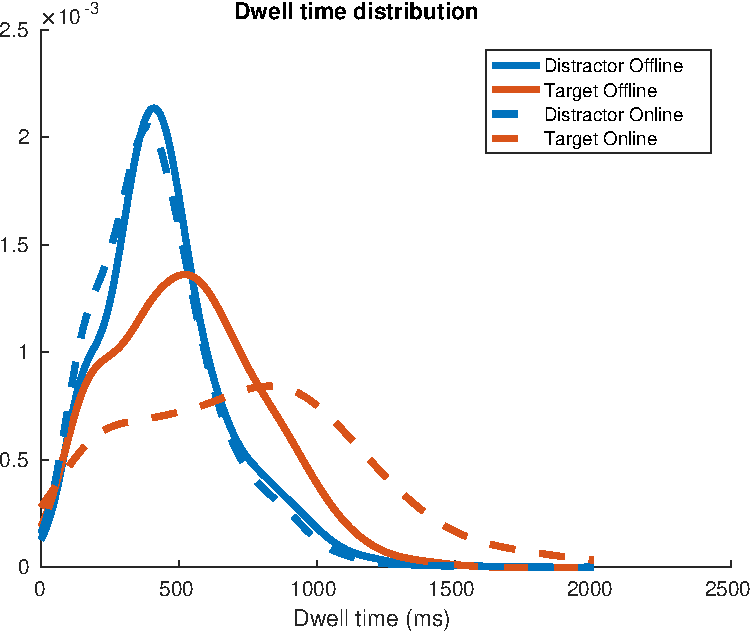
\includegraphics[trim={0cm 0cm 0cm 0cm},clip,width=0.6\columnwidth]{../images/DwelltimeDist_online_allmean.pdf}
    \caption{Dwell time distribution for first dwells on
    targets vs distractors in offline and online phases. The single-subject
    distributions were smoothed and averaged across subjects.}
\label{fig:dwell}
\end{figure}

\subsection{EFRP waveform}
\begin{figure}[!t]
    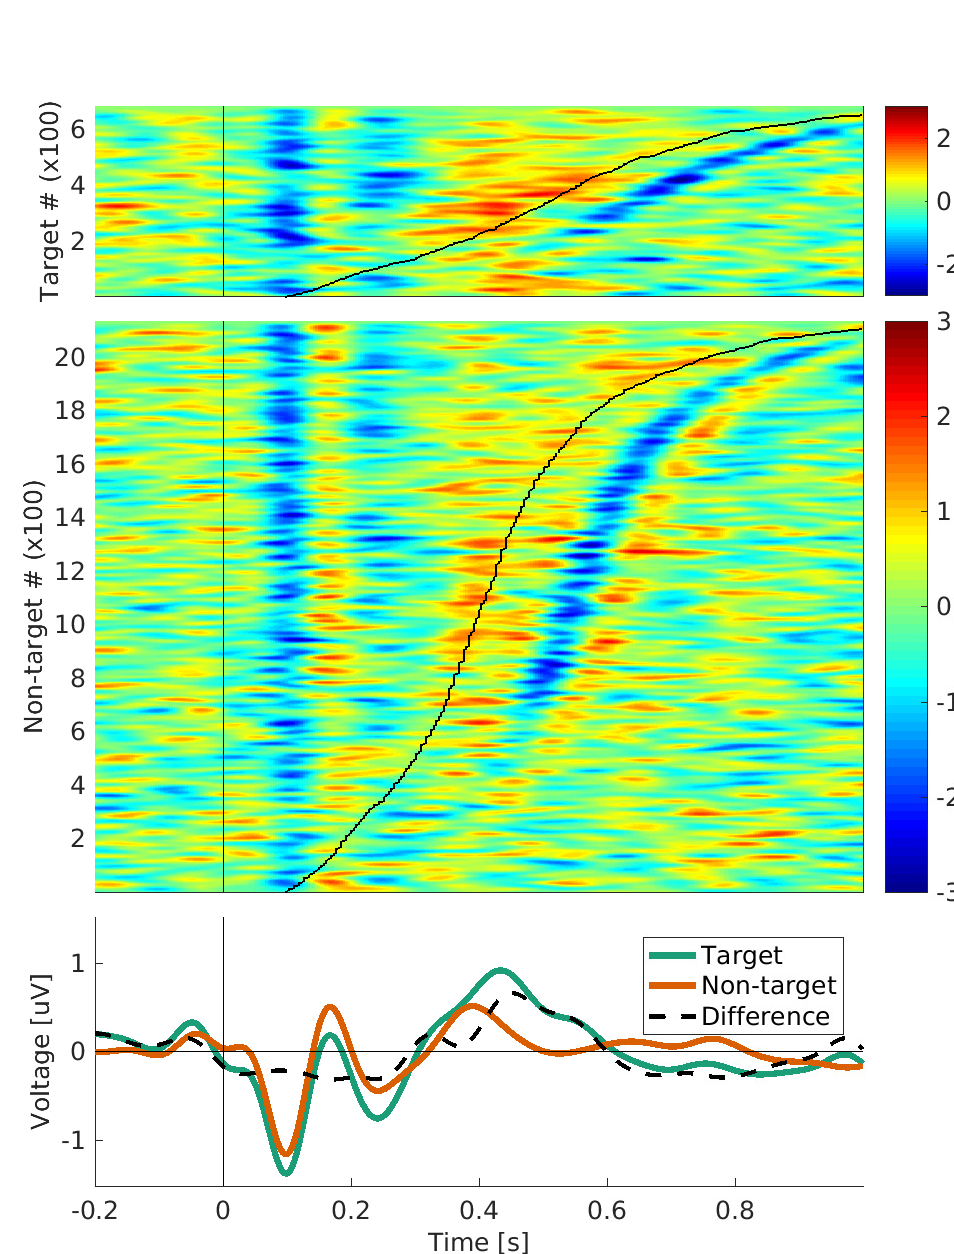
\includegraphics[trim={0cm 0cm 1.5cm 0cm},clip,width=0.45\columnwidth]{../images/offline/Epochs_GA_chCz_Saggregate_objrec_subjects_popuponline_s1.pdf}
    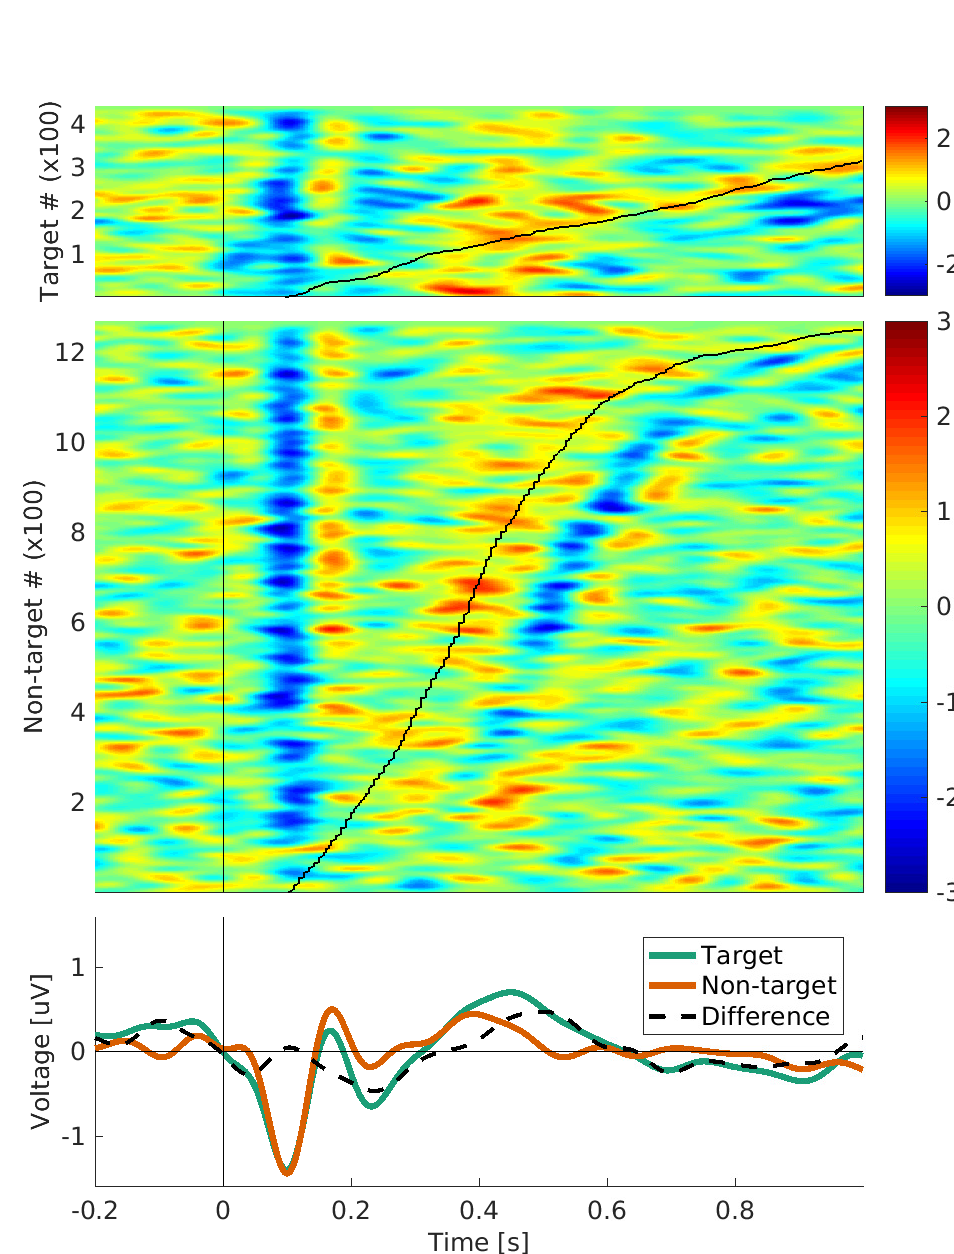
\includegraphics[trim={0cm 0cm 1.5cm 0cm},clip,width=0.45\columnwidth]{../images/online/Epochs_GA_chCz_Saggregate_objrec_subjects_popuponline_s1.pdf}
    \caption{The signal of Cz channel for extracted epochs aggregated
        for the 4 best performing subjects with PLR-Waveform approach.
        Left: offline, Right: online.
        The epochs are ordered according to the dwell time
        shown with the black curve.
    }
\label{fig:epochsCz}
\end{figure}

\begin{figure}[!t]
    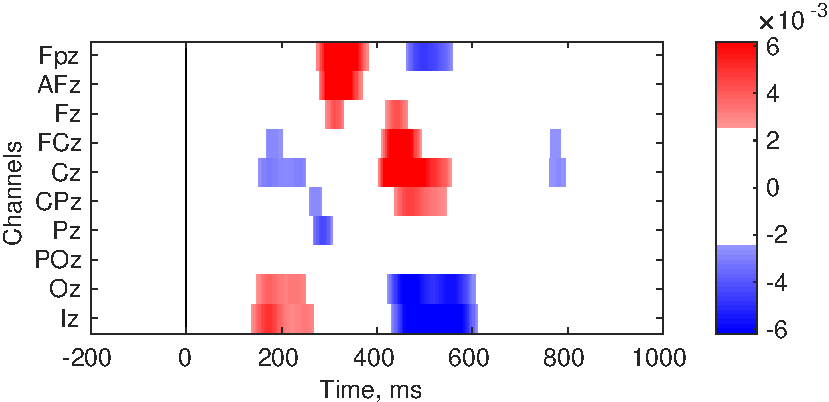
\includegraphics[trim={0cm 0.01cm 0cm 0cm},clip,width=0.45\columnwidth]{../images/SignR_offline.pdf}
    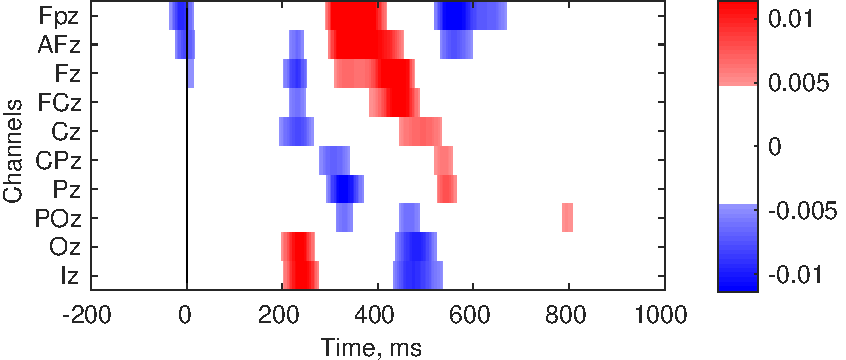
\includegraphics[trim={0cm 0cm 0cm 0.01cm},clip,width=0.45\columnwidth]{../images/SignR_online.pdf}
    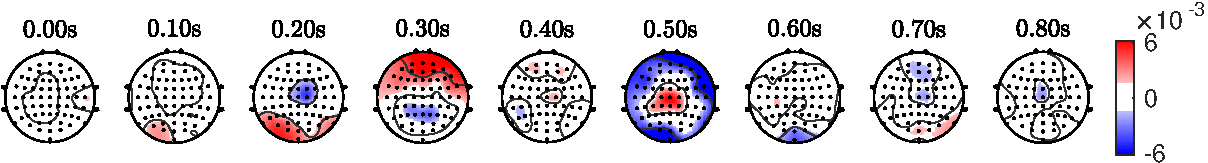
\includegraphics[trim={0cm 0cm 0cm 0cm},clip,width=0.9\columnwidth]{../images/offline/TopoPlot_TLock-start_signRSquare_Saggregate_objrec_subjects_popuponline_s1.pdf}
    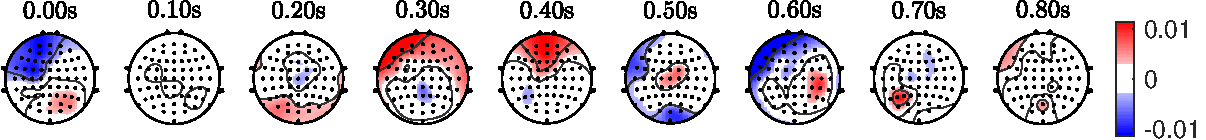
\includegraphics[trim={0cm 0cm 0cm 0cm},clip,width=0.9\columnwidth]{../images/online/TopoPlot_TLock-start_signRSquare_Saggregate_objrec_subjects_popuponline_s1.pdf}
    \caption{The discriminant power for the aggregated epochs of
        4 best subjects with the offline AUC above 0.6 with PLR-Waveform approach.
    Signed $R^2$ is demonstrated for midline channels across around the eye fixation onset
    (top left: offline, top right: online) and on topographic maps (top map: offline, bottom map: online).}
\label{fig:signR}
\end{figure}


We present the analysis of the aggregated EFRP waveform
for the 4 subjects who demonstrated
the highest classification performance in the offline phase with the 
PLR-Waveform classifier because it allows for direct representation
of the features used by a linear classifier (see Section \ref{sec:class}).

We visualized the representative Cz channel signal
for each eye fixation while ordering them
by the dwell time (Figure \ref{fig:epochsCz}).
The amplitude of the presented EFRP is limited to the range [-1.5, 1.5] uV.
The complex of components right after the fixation onset ranging from 100 to 300 ms
reflects the evoked potentials from the fixation itself. It contains
negative and positive deflections. We can observe the same complex of components
after the dwell offset. The shift of gaze happens right where we expect 
the P300-like component so it can be masked by this evoked activity.
The positive deflection occurs at the end of the dwell for both
targets and non-targets, however it has a greater amplitude for targets
as seen on the averaged EFRP.

The univariate discriminant power is shown on the Figure \ref{fig:signR}.
The results are similar for the offline and online phases, with online data having twice
as higher discriminant power with up to 0.01 of signed $R^2$.
The greatest values are mainly confined within the region between 100 and 700 ms.
The higher discriminant power is spread across the whole scalp which can be the consequence
of using CAR in the processing. Nonetheless, the P300-like component of EFRP can be seen at 500 ms
after the fixation onset.



\subsection{Comparison of decoding approaches}
\label{sec:class}

\begin{figure}[!t]
    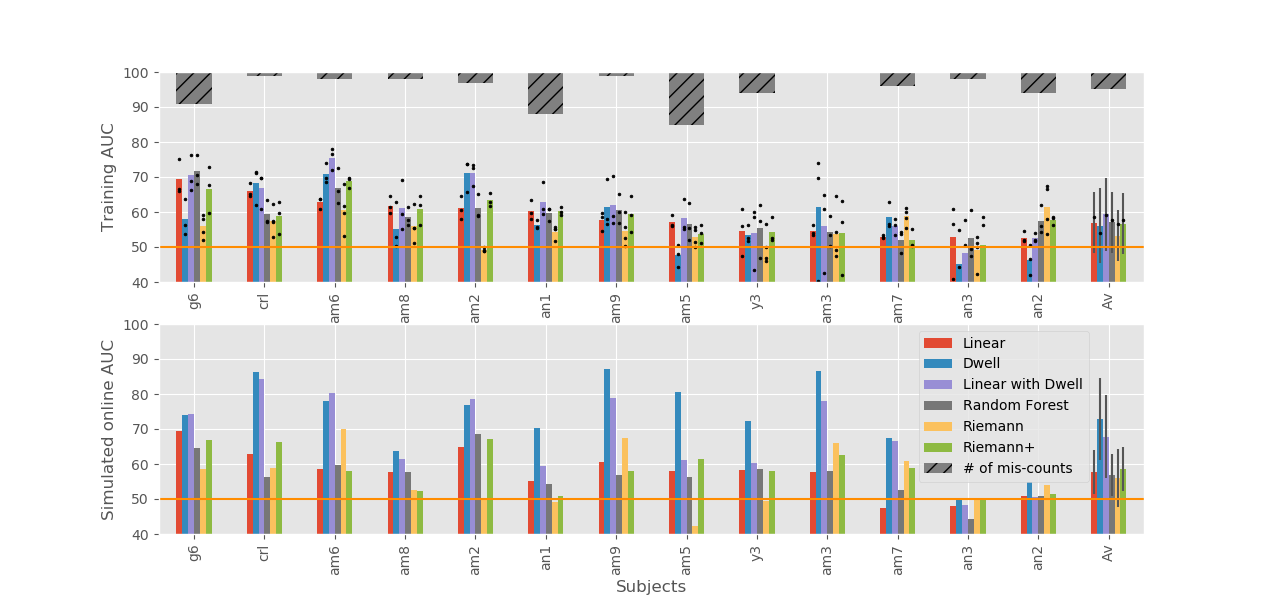
\includegraphics[trim={2cm 0cm 2cm 0cm},clip,width=1.1\columnwidth]{../images/ClassificationAll.png}
    \caption{Performance of EFRP classification with various approaches in offline analysis (top)
    and simulated online analysis (bottom) as percentage of AUC.
    Each dot shows single fold performance
    in a leave-one-run-out cross validation for the corresponding classification approach.
    The overlaid gray bars at the top show the behavioral performance:
    the number of mis-counts in offline phase on the same scale as AUC percentage.}
\label{fig:classAll}
\end{figure}

\subsubsection*{Offline}
All the classification methods yielded a single-trial 
performance between 0.53 and 0.6 AUC on average
(Figure \ref{fig:classAll})
which is statistically significant against random level of 0.5 
for all methods except PLR-Dwell
(p-values $< 0.01$ with Student's t-test after Bonferroni correction
for 6 methods).
Eight out of thirteen subjects achieve performance 
above 0.6 for at least one of the approaches based
on EEG features.
Performance of different approaches has a different ranking per subject, however
the differences between
the approaches are not statistically significant (p-value $= 0.16$ with repeated measures ANOVA).
It is worth noticing that the combination of both dwell time and EEG waveform is not always
better than just one of these feature sets.

\subsubsection*{Simulated online}
It is worth noting that the performance of EEG-based approaches
on online data is consistent with the training performance on offline data.
The average AUC values lie between 0.56 and 0.59 for each approach
which is statistically significant against 0.5
for all approaches except PLR-Riemann.
(p-values $< 0.01$ with Student's t-test after Bonferroni correction 
for 6 approaches).

For approaches relying on the dwell time, however, the performance drastically improved
for multiple subjects compared to the offline performance.
The average AUC for \textit{dwell} classifier increased
from 56 to 73 and for the \textit{PLR-Combined} classifier from 59 to 67.
This improvement is a direct consequence of the increased target dwell time
together while non-target dwell time remained unchanged, see Figure \ref{fig:dwell}.
However, the underlying question of why the dwell time changed 
between the offline and the online phases still remains.


\subsection{Online performance}

\begin{figure}[!t]
    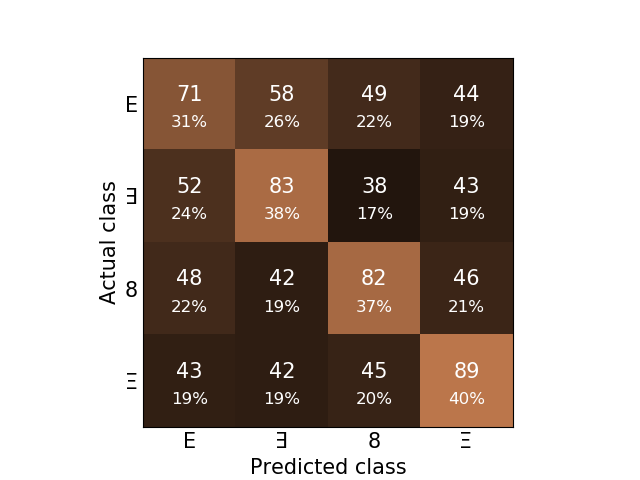
\includegraphics[trim={1cm 0cm 1cm 1cm},clip,width=0.7\columnwidth]{../images/OnlineConfusion_percent.png}
    %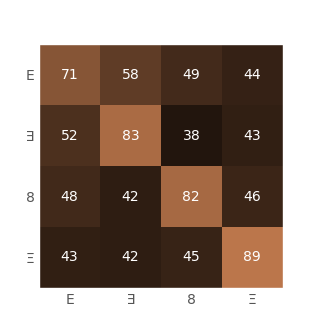
\includegraphics[trim={0cm 0cm 0cm 0cm},clip,width=0.5\columnwidth]{../images/OnlineConfusion.png}
    \caption{The aggregated confusion matrix of online decoding for each type of symbol being
    a target class. The absolute number of cases is presented and normalized as percentage 
    relative to the actual class (row-wise normalization).}
\label{fig:onlineconf}
\end{figure}


\begin{table}
    \centering
    \caption{Online performance. The test results show the p-values after Benjamini-Hochberg correction.
    Statistically significant results are typed in bold.}
    %\tiny
    %\footnotesize
    \scriptsize
    \renewcommand{\arraystretch}{1.5}
    \begin{tabular}{l r r r r r r r r r r r r r}
        \hline
        Subjects & S1 & S2 & S3 & S4 & S5 & S6 & S7 & S8 & S9 & S10 & S11 & S12 \\
        \hline

        Accuracy & 0.44 & 0.38 & 0.45 & 0.29 & 0.44 & 0.35 & 0.39 & 0.25 & 0.31 & 0.38 & 0.38 & 0.4 \\ 
        %0.44, 0.38, 0.45, 0.29, 0.44, 0.35, 0.39, 0.25, 0.31, 0.38, 0.38, 0.4
        \shortstack{Accuracy \\ test} & \textbf{0.001} & \textbf{0.04} & \textbf{0.001}
        & 0.48 & \textbf{0.001} & 0.07 & \textbf{0.02} & 1.0 & 0.24 & \textbf{0.04} & \textbf{0.04} & \textbf{0.03} \\
        \shortstack{Independence \\ test}  & \textbf{0.004} & 0.29 & \textbf{0.03} & 0.74
        & 0.08 & 0.17 & 0.1 & 0.41 & 0.48 & 0.19 & 0.22 & 0.26 \\
        \hline
        % Benjamini/Hochberg
        %All chi:  [0.0044, 0.2867, 0.0304, 0.7427, 0.081, 0.169, 0.0978, 0.4127, 0.4781, 0.1904, 0.2193, 0.2596]
        %All binom:  [0.001, 0.0363, 0.001, 0.4794, 0.001, 0.0688, 0.0193, 1.0, 0.2405, 0.0363, 0.0363, 0.0318]
        % Bonferroni
        %Binom:  [0.003, 0.2903, 0.0016, 5.2731, 0.003, 0.6192, 0.0771, 12.0, 2.4047, 0.2903, 0.2903, 0.1592]
        %Chi * 12  [0.0044, 2.5806, 0.0608, 8.9126, 0.243, 0.8449, 0.3913, 4.1269, 5.2593, 1.1424, 1.5352, 2.0768]
    \end{tabular}
    \label{tab:onlineperf}
\end{table}

We assessed the task performance for each subject as the accuracy of
decoding target at the end of the road integrated after multiple presentations
of each type of boards (Table \ref{tab:onlineperf}).
The averaged accuracy 
equals 0.37 and it is significantly different from random level of 0.25 for
a multi-class classification with 4 balanced classes (p-value $< 0.0001$ with Student's t-test).
Additionally, we applied statistical test to assess the accuracy per subject.
After adjusting p-values with Benjamini-Hochberg procedure 8 subjects performed statistically above chance level.

To verify the independence of the 4 classes in online phase
we computed the aggregated confusion matrices across all symbols for all subjects (Figure \ref{fig:onlineconf}).
We applied an independence test for confusion matrices per subject.
After adjusting p-values with Benjamini-Hochberg procedure
only two subjects show significant imbalance in the
confusion matrix. It is linked to a high accuracy of the symbol $\Xi$ and low accuracy 
for the symbol E.


\section{Discussion}
\label{sec:discussion}

The integration of the BCI systems in daily life of 
healthy/able-bodied users requires the system 
to be built around the experimental paradigms
 supporting human natural behavior.
To this end, EFRP-based decoding of cognitive 
processes in overt visual search has a potential
to augment human-machne-interaction. 
In this study we investigated the decoding of visual recognition in a driving scenario.
It resembles one of the typical everyday activity
and provides the associated challenges in decoding visual recognition:
free eye gazes, dynamic visual input, primary tasks.
For this purpose we limit the driving task to following 
the simple route at a comfortable and natural speed.
To avoid overloading subjects' attention with too many distractors,
we did not include other participants on the road nor moving objects.
Nonetheless, due to the movement of the car, the drivers
were subjected to a dynamic visual input and perceived a
natural optic flow.

\subsubsection*{Ocular behavior in driving.}
We considered random pop-up appearance of the task relevant
stimuli above the sidewalks.  In the previous study
on active search in dynamic scene \cite{uscumlic_active_2016},
this type of appearance created sufficient locking
of the cognitive EFRP's components to the fixation onset.
At the same time, their results showed that the time spent
on the stimuli was not informative about
the stimuli type (target vs. non-target) in contrast
to the more attentionally demanding motion appearance conditions.   
Interestingly, we observed  the time spent on the stimuli  to be
discriminative in our exp. scenario although the same
pop-up stimuli appearance was considered.
This illustrates the effect of the user/driver motion
relative to the visual content on the visual information
processing and the attentional load. Moreover, in the online phase
subjects looked longer on targets compared to the offline phase.
Although the subjects dwell time was not decoded directly, they were aware
that they could potentially influence the decoding quality. This might
lead to deliberate or unconscious changes in their behavior.
Some subjects could achieve a high decoding performance based
only on dwell time in offline phase. But with the changes in the behavior
during online phase, most of the subjects drastically improve in their decoding performance
based on the dwell time.


The board attendance rate reveals two aspects of the task completion:
(1) how well the subjects coped with the pace and attentional load
and (2) whether they can differentiate between targets and distractors
using their peripheral vision.
We observed a statistically significant difference in the board attendance
between offline and online phases despite the equal number of boards.
On one hand, we expected the subjects to 
be more engaged in the task due to interactive feedback part.
However, the observed increase of the dwell time on target boards 
in online phase made it more challenging to attend all
the boards within the limited time.
On the other hand, behavioral response based on number of recognized targets
were not required which might relax the cognitive load.

We carefully designed stimuli
to ensure that their recognition requires foveal vision.
It is confirmed by similar
attendance rate on targets and non-targets and 
by just a few errors in the counting task.
We were concerned that the introduction of new symbols in the online phase
may change the behavior or the cognitive response due to the novelty.
The balanced confusion matrices of decoding target recognition in the online phase
confirm that subjects perceived all the symbols equally with regards
to the task. However, the presence of additional types of stimuli 
may have contributed to the increased dwell time 
on the target boards because the target identification among 4
categories is more challenging than among 2 categories
\cite{dick_processing_1971,alegria_time_1970}.


\subsubsection*{Decoding visual recognition in driving.}
The discriminant analysis of EFRP shows similar results for both
offline and online phases. Most of the relevant
features lie within [200, 700] ms window which coincides with the dwell
durations. The spatial localization of relevant features is consistent with the typical
spatial distribution of P300 component in oddball paradigm.
The EFRP waveforms are known to contain a strong P1 component at the occipital
area that reflects the beginning of the visual processing of a stable visual input
after the saccade. In the analysis of Cz channel, it corresponds to the negative
deflection at 100 ms. It is clearly present in most of the first fixations on boards.
Moreover, we could also see it for the following fixations.
During the dwell time multiple fixations can be detected 
what leads to the overlap of the P300-like component
locked to the 1st fixation and the following early EFRP component.
In contrast to the classical P300 paradigms where the timing
of the visual input is controlled (regular timing), here the
overlap of EFRP are variable across trials.
This is an additional challenge as compared to typical
event-related potential detection approaches.
%It leads to the overlap between P300-like component and 
%the evoked fixation-related components. This overlap contaminates the
%data and complicates the decoding of cognitive process.
Removing the activity related to previous and subsequent fixations
from the EEG was attempted by modeling it from
various characteristics of the previous and subsequent fixations.
\cite{devillez_p300_2015,devillez_eye_2015,kristensen_comparison_2015}.
We did not choose to apply this approach as there is a risk 
to distort the signal of interest.
The precise EFRP shape depends on preceding and following
eye behavior (e.g. amplitude and direction of the saccades)
as well as low-level features of the visual input
\cite{nikolaev_combining_2016}.

%We limited the removal of artifacts to high frequency spatial noise with SPHARA 
%and direct eye movement potential propagation by regressing it out 
%from the EOG signal.

We compared multiple classification approaches based on EFRP on offline data and 
simulated their application to online data.
All approaches, including waveform-based linear and non-linear and covariance-based 
methods, resulted in similar performance on average across subjects
which is significantly above the chance level for most
of the approaches.
However, there is no single best approach for all subjects.

The actual online performance in closed-loop measured by the target symbol identification
is significantly above the chance level only for 3 subjects.
Nonetheless, on average across subjects the accuracy of 0.37 is 
significantly higher than 0.25.

One can argue that the high performance of EFRP-based classifiers is
due to the strong and well-aligned evoked potentials after the fixations offset,
which reflects the difference between the target and non-targets dwell times.
In this case we would see an improvement in performance for online data
similar to the classification approaches based on dwell time.
A simple concatenation of features from two sources 
of information (EEG and dwell time), nonetheless,
does not lead to significant improvement and in the simulated online,
such a decoding results in intermediate performance.
In this study our primary goal was to explore the neural correlates
of the object recognition.
Ocular correlates such as pupil dilation along with multi-modal
integration of neural and ocular correlates may be further investigated
in future studies.
Multimodal integration may improve the decoding performance \cite{jangraw_neurally_2014}.


\section{Conclusion}
\label{sec:conclusion}


In this study we demonstrated the feasibility to decode
recognition of visual targets from brain signals in challenging conditions
of everyday driving scenario.
The system can be validated in a specific application
of realistic interaction between the driver and the car.
For example, the achieved decoding performance 
might be enough to recognize subjectively interesting
categories of road signs and objects and provide valuable recommendations
to drivers.
Further improvements can be introduced in different parts
of the system before specific application testing,
such as higher quality eye-tracker with a real-time
implementation of robust segmentation algorithm,
longer training of subjects over multiple sessions,
and multimodal integration of neural
and ocular data.

\ack

The authors thank Nissan Motor Co. Ltd for supporting
this work.

\section*{References}

\bibliographystyle{unsrt}
\bibliography{ObjRec_DS}

\end{document}

